\begin{frame}{3º Ciclo}
	\begin{columns}
		\column{.3\textwidth}
        Ciclo Impacto
		\column{.7\textwidth}
		\begin{figure}[hb]
      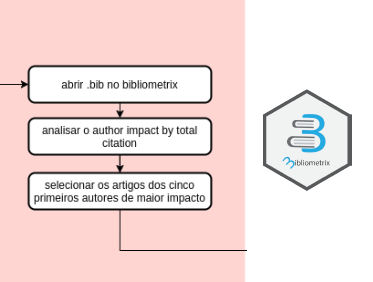
\includegraphics[width=0.9\textwidth]{figures/ciclo3.png}
		\end{figure}
	\end{columns}
\end{frame}

\begin{frame}{3º Ciclo}
  Analisar o Author Impact
	\begin{figure}[hb]
    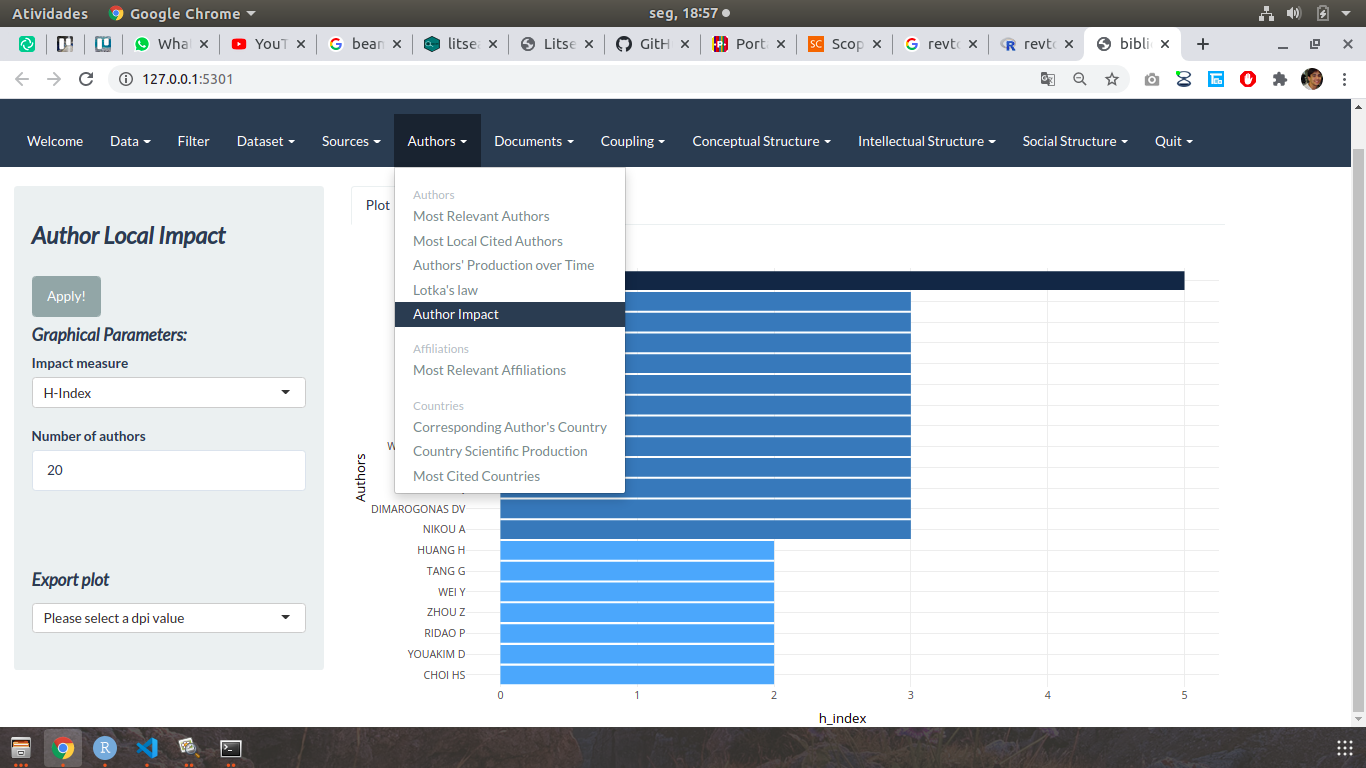
\includegraphics[width=1\textwidth]{figures/autorimpact1.png}
  \end{figure}
\end{frame}

\begin{frame}{3º Ciclo}
  Analisar o Author Impact by Total Citation
	\begin{figure}[hb]
    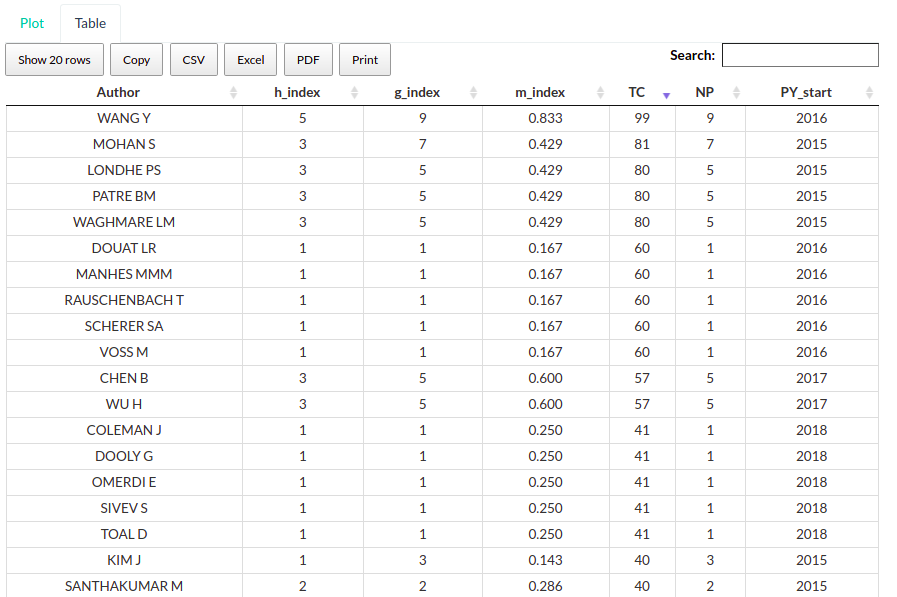
\includegraphics[width=0.8\textwidth]{figures/autoimpact2.png}
  \end{figure}
\end{frame}

\begin{frame}{3º Ciclo}
  Selecionar os artigos dos cincos primeiros autores de maior impacto
	\begin{figure}[hb]
    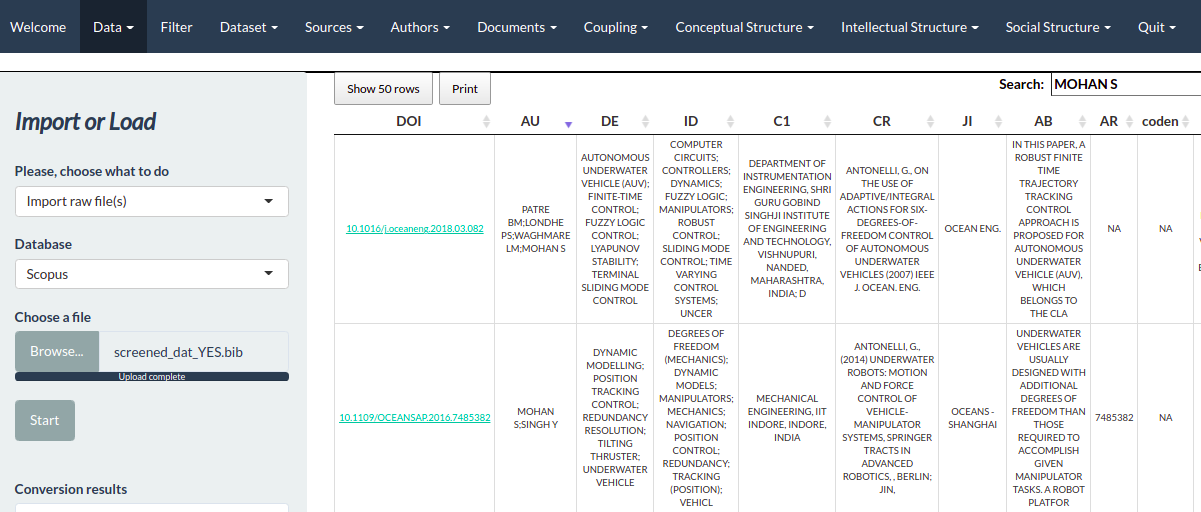
\includegraphics[width=1\textwidth]{figures/buscarartigo.png}
  \end{figure}
\end{frame}

\begin{frame}{4º Ciclo}
	\begin{columns}
		\column{.3\textwidth}
        Ciclo de Produção
		\column{.7\textwidth}
		\begin{figure}[hb]
      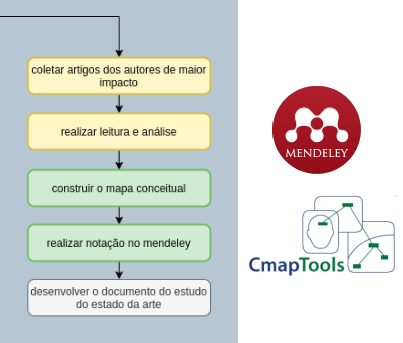
\includegraphics[width=0.8\textwidth]{figures/ciclo4.png}
		\end{figure}
	\end{columns}
\end{frame}

\begin{frame}{Mendeley}
	Conhecido pelo gerenciador de referências, usado para gerenciar, compartilhar e criar referências bibliográficas para artigos acadêmicos.

	\begin{figure}[hb]
		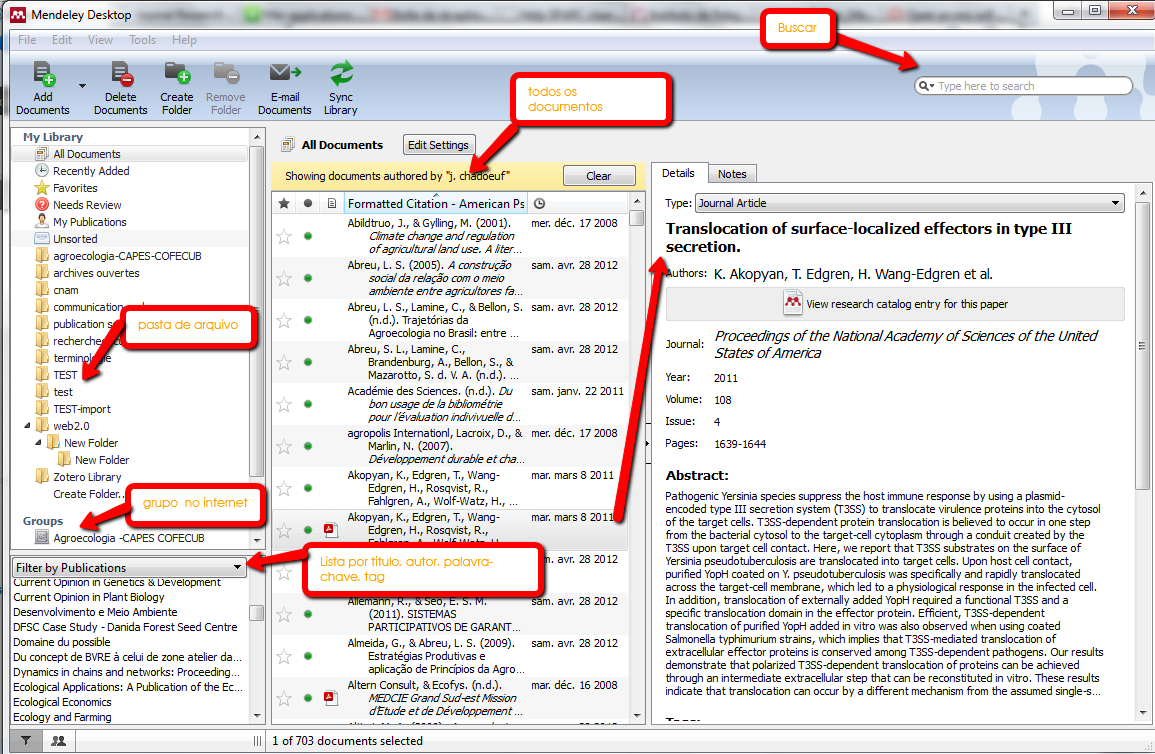
\includegraphics[width=0.8\textwidth]{figures/mendeley.png}
	\end{figure}
\end{frame}

\begin{frame}{CmapTools}
	Software de mapeamento de conceito

	\begin{figure}[hb]
		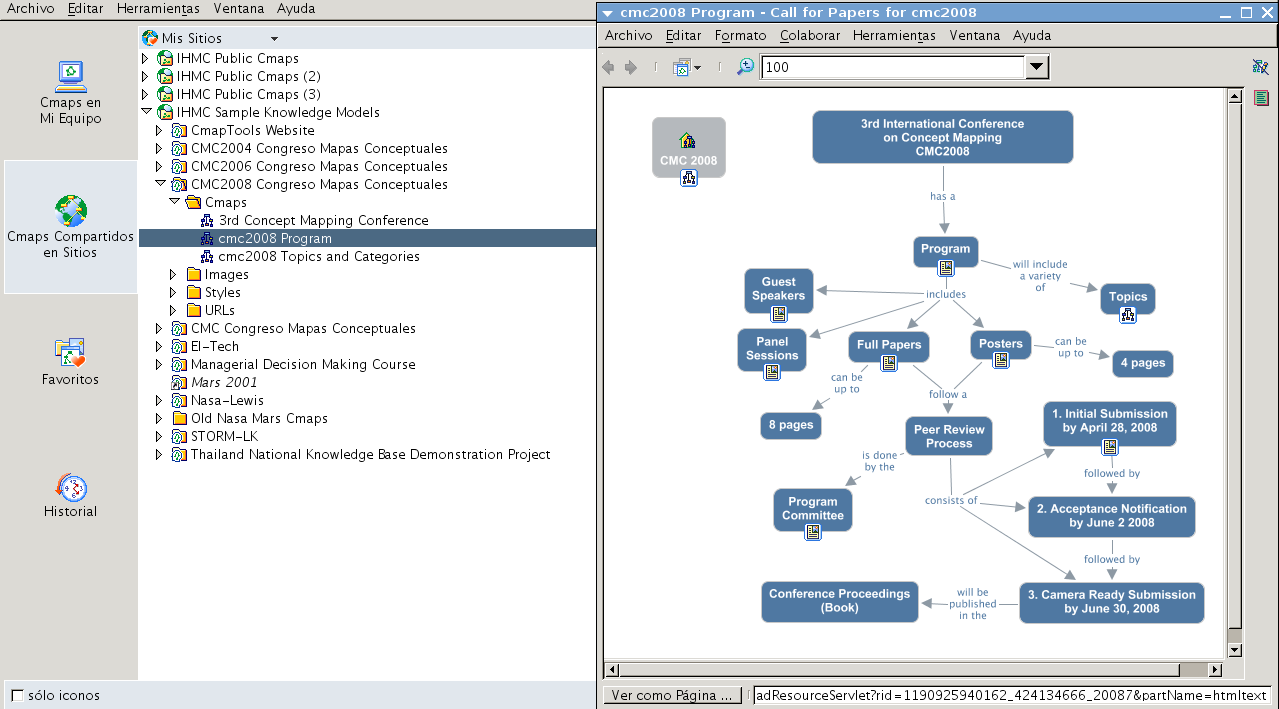
\includegraphics[width=0.8\textwidth]{figures/cmaptools.png}
	\end{figure}
\end{frame}